\chapter{Track Occupancy Detector Extension Board}

Track occupancy detectors are essential for building any block control or layout automation. The key idea is to divide the track into sections and then monitor each section for current consumption. The basic principle has been described in the power module chapter. When a locomotive is on the track section a current is flowing and there is a voltage drop along the diodes which is translated to a signal. With a DCC signal on the line, this task is straightforward, there is always a current flowing. In an analog track section, a stopped loco does not draw current. In such cases a very small current is sent periodically, enough to trigger the sensors but not enough to move anything.

\section{Block Diagram}

\begin{figure}[htbp]
    \centering
    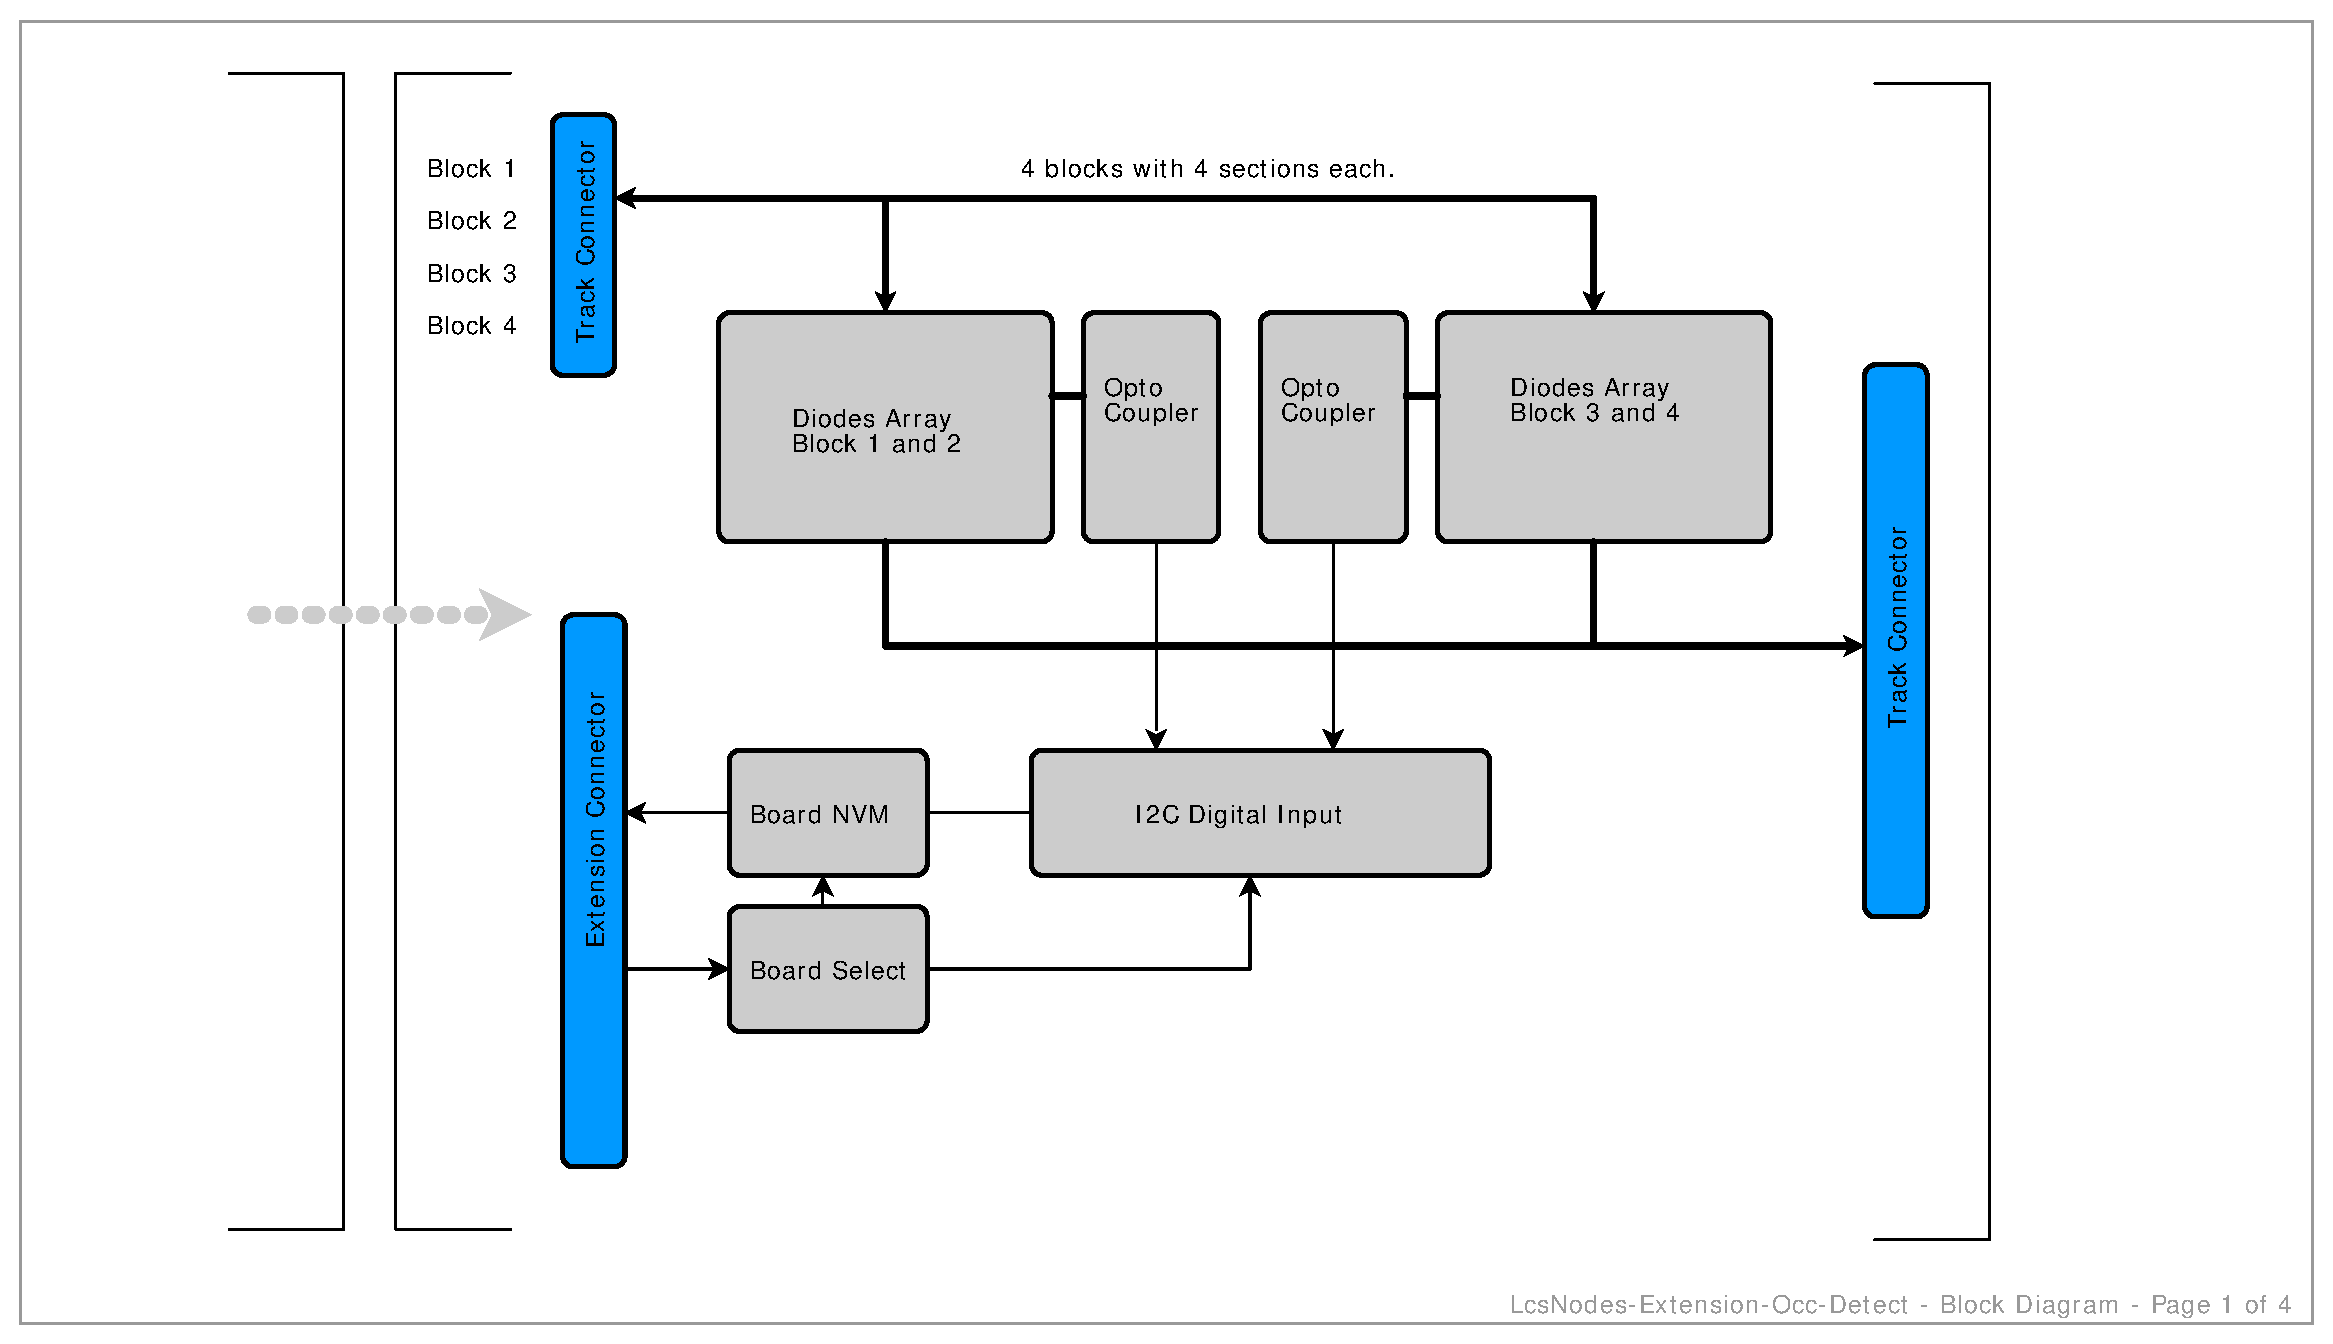
\includegraphics[page=1, width=0.9\textwidth]{./Schematics/Schematic_LcsNodes-Extension-4x4-Occ-Detect.pdf}
    %\label{fig:schematic}
\end{figure}
\FloatBarrier

\section{Connectors and Logic}

\begin{figure}[htbp]
    \centering
    \includegraphics[page=2, width=0.9\textwidth]{./Schematics/Schematic_LcsNodes-Extension-4x4-Occ-Detect.pdf}
    %\label{fig:schematic}
\end{figure}
\FloatBarrier

\section{Detectors}

The sensor detector uses bridge rectifiers instead of discrete diodes. This allows for a rather dense packing. Bridge rectifiers are available for up to two Amps, which will be fine for a HO or smaller gauge layout. For the large scales the sensor needs to be built using discrete diodes, such as the SB560 Schottky Diode. Note also that the power for the track is not routed via the main controller board. The track power is directly connected to the extension board.

\begin{figure}[htbp]
    \centering
    \includegraphics[page=3, width=0.9\textwidth]{./Schematics/Schematic_LcsNodes-Extension-4x4-Occ-Detect.pdf}
    %\label{fig:schematic}
\end{figure}
\FloatBarrier

\begin{figure}[htbp]
    \centering
    \includegraphics[page=4, width=0.9\textwidth]{./Schematics/Schematic_LcsNodes-Extension-4x4-Occ-Detect.pdf}
    %\label{fig:schematic}
\end{figure}
\FloatBarrier

\section{PCB}

\section{Block Diagram}

\begin{tikzpicture}[scale=0.9, transform shape]

    \draw[help lines, gray!50, dashed] (0,0) grid( 16,8);
    \node at (8,4) {picture};

\end{tikzpicture}


\section{Firmware}

\begin{itemize}
\item I2C address considerations
\item nodes and port attributes, which ones are common to all sensors ?
\item periodically scan each section
\item events could be fired
\item control and info items to access, every group is one port
\end{itemize}

\section{Summary}

